76. Приложить друг к другу два прямоугольника можно тремя способами. В первых двух случаях прямоугольники одинаковые, а в третьем --- это прямоугольники $4\times1$ и $16\times4$(он тоже имеет пузатость $4:1$). Получим пузатости $8:1,\ 2:1,\ 17:4.$
\begin{center}
\begin{figure}[ht!]
\center{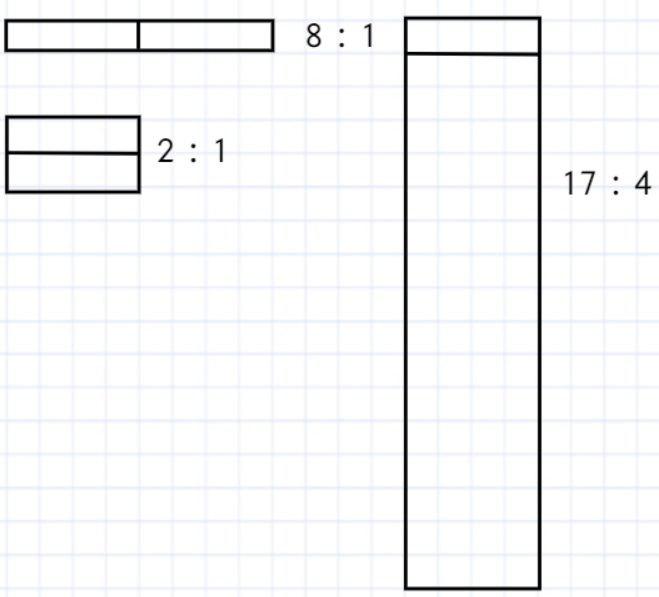
\includegraphics[scale=0.35]{puz1.png}}
\end{figure}
\end{center}
